%% ============================================================
%%  JAIR-format version.
%%  HOW TO USE (important):
%%  1. Download the JAIR author kit (the .zip in the rejection
%%     letter / https://www.jair.org/index.php/jair/libraryFiles/
%%     downloadPublic/6). It contains jair.cls + the template +
%%     the reproducibility checklist.
%%  2. On Overleaf, create a project from that kit zip.
%%  3. Upload the /figures folder into that project.
%%  4. Replace the kit template's TITLE, AUTHORS, ABSTRACT, BODY,
%%     and REFERENCES with the ones below (keep the kit's
%%     reproducibility-checklist appendix and set the answers
%%     given separately in the chat).
%%  jair.cls is required; this file will NOT compile without it.
%% ============================================================
\documentclass{jair}
\usepackage{amsmath,amssymb}
\usepackage{graphicx}
\usepackage{tikz}
\usetikzlibrary{arrows.meta,positioning}
\usepackage{algorithm}
\usepackage{algpseudocode}

\title[Trustworthy Skin-Lesion Screening on Real-World Images]{Does It Know When It Is Wrong? Classification versus Retrieval for Trustworthy Skin-Lesion Screening on Degraded and Real-World Images}

\author{Nishan Kharel}
\affiliation{%
  \institution{Institute of Science and Technology, Tribhuvan University}
  \city{Kathmandu}
  \country{Nepal}}
\email{nkharel57@gmail.com}

\author{Paras Simkhada}
\affiliation{%
  \institution{University of Greenwich}
  \city{London}
  \country{United Kingdom}}
\email{simkhadaparash@gmail.com}

\renewcommand{\shortauthors}{Kharel \& Simkhada}

\begin{abstract}
\textbf{Background:} Deep networks match dermatologists on curated skin-lesion
images, but are almost always trained and tested on clean, dermatoscopic
photographs. In deployment---especially phone-based screening where a specialist
is far away---inputs are blurry, dark, compressed, or captured with an ordinary
camera, and a screening tool that fails silently on them is dangerous.

\textbf{Objectives:} We ask a trust-centred rather than accuracy-centred
question: on degraded and real-world images, which design is more reliable, a
fine-tuned classifier or an embedding-based case-retrieval model, judged jointly
by robustness of the malignant class and by honesty of its own uncertainty.

\textbf{Methods:} Using HAM10000 we compare an EfficientNet-B0 classifier
against DINOv2 nearest-neighbour retrieval under a graded corruption suite and,
with no retraining, on 2{,}106 real smartphone photographs from PAD-UFES-20,
reporting bootstrap 95\% confidence intervals throughout. We ablate the
retrieval confidence signal and analyse errors via retrieved cases.

\textbf{Results:} Aggregate accuracy hides a melanoma-sensitivity collapse:
under low light and noise the classifier's melanoma recall falls to near zero
while retrieval holds at 40--50\%. A distance-based retrieval confidence,
calibrated on degraded validation data, is the best-calibrated model even under
heavy corruption (ECE 0.03), whereas vote share is badly overconfident
(0.23--0.31). On real smartphone photos retrieval catches $3.5\times$ more
melanomas (0.40 vs.\ 0.115, non-overlapping CIs) and detects the distribution
shift (AUROC 0.94 vs.\ 0.72). Confidence-based abstention does not raise
melanoma recall, an honest negative showing calibration and ranking differ.

\textbf{Conclusions:} A retrieval design with the right uncertainty signal is
simultaneously more robust and more honest about what it does not know, while
aggregate accuracy conceals the classifier's silent melanoma failures. Overall
accuracy under the real modality shift is low for both models, as expected;
trust, not clean-set accuracy, should drive evaluation of screening models.
\end{abstract}

\keywords{skin cancer, melanoma, medical image analysis, robustness,
distribution shift, calibration, uncertainty estimation, image retrieval,
out-of-distribution detection, trustworthy AI}

\maketitle

\section{Introduction}
Melanoma is the deadliest common skin cancer and early detection sharply
improves survival. Convolutional networks now rival dermatologists on benchmark
data~\citep{esteva2017}, and datasets such as HAM10000~\citep{tschandl2018} and
the ISIC challenges~\citep{codella2018} have driven rapid gains. Almost
universally, however, models are evaluated on \emph{clean, dermatoscopic}
images. The photographs a real person submits---on a phone, often blurry, dark,
tilted, or compressed---look nothing like that training distribution.

The failure mode is not merely lower accuracy but \emph{silent} failure: a model
that outputs ``benign, 95\% confident'' on a degraded melanoma tells a patient
not to seek care. For a screening tool meant to widen access where
dermatologists are scarce, the right question is not only ``how accurate?'' but
``does it know when it is wrong?''

We compare two designs on identical data and evaluation: a \textbf{classifier}
(fine-tuned EfficientNet-B0) and a \textbf{retrieval} model (frozen DINOv2
embedding, classified by a weighted vote over nearest stored cases, whose
distance to those cases is itself an uncertainty signal). We evaluate under a
graded corruption suite and, crucially, on real smartphone photographs from
PAD-UFES-20~\citep{pacheco2020}, with no retraining.

\noindent\textbf{Contributions.}
\begin{itemize}
\item A head-to-head comparison of classification and retrieval on the axes that
matter for trust---robustness of the \emph{malignant} class and honesty of
confidence---with bootstrap confidence intervals.
\item Evidence that aggregate accuracy \emph{masks} a melanoma-sensitivity
collapse under degradation.
\item The finding that a retrieval model's calibration under distribution shift
hinges on the confidence signal: a distance-based, shift-calibrated confidence
stays well-calibrated (ECE $\approx0.03$) under heavy corruption.
\item A real-world validation on smartphone photographs, where retrieval catches
significantly more melanomas and detects the shift.
\item An honest negative on selective prediction, distinguishing calibration
from ranking, plus interpretable case-based error analysis.
\end{itemize}

\section{Related Work and Gaps}
\textbf{Skin-lesion classification.} From dermatologist-level
classification~\citep{esteva2017} to standardised
benchmarks~\citep{tschandl2018,codella2018}, accuracy on clean dermoscopy has
risen; foundation models push further---DINOv2~\citep{oquab2024dinov2},
BiomedCLIP~\citep{zhang2025biomedclip}, and dermatology-specific
PanDerm~\citep{yan2025panderm}. \emph{Gap:} evaluation is almost always on clean
in-distribution data, rarely characterising class-specific behaviour under
degradation.

\noindent\textbf{Robustness and shift.} Common-corruption robustness was
formalised for natural images~\citep{hendrycks2019} and adapted to
dermoscopy---a skin-cancer robustness benchmark~\citep{maron2021}, corruption
suites with test-time adaptation~\citep{hu2024diffusion}, artifact-driven domain
generalisation~\citep{bissoto2022artifact}, and modality-aware
corruptions~\citep{disalvo2024medmnistc}. \emph{Gap:} results are aggregate,
obscuring class-specific clinical risk, and rarely compared across paradigms.

\noindent\textbf{Calibration and uncertainty.} Modern networks are
miscalibrated~\citep{guo2017}; ECE~\citep{naeini2015} and isotonic
regression~\citep{zadrozny2002} quantify and correct this. In medical imaging:
conformal prediction for skin lesions~\citep{fayyad2024conformal}, calibration
robust to label noise~\citep{penso2024calibration}, and drivers of
calibration~\citep{sambyal2023understanding}. \emph{Gap:} calibration is
typically assessed in-distribution, and honest confidence for a \emph{retrieval}
model under shift is unexplored.

\noindent\textbf{Retrieval and case-based diagnosis.} CBIR and $k$-NN over deep
embeddings offer transparency: saliency-enhanced CBIR for
dermatology~\citep{gassner2023secbir}, nearest-neighbour search on pretrained
features~\citep{gupta2023mednn}, and metric learning for
dermoscopy~\citep{he2022demal}. \emph{Gap:} retrieval is seldom pitched
head-to-head against a classifier as a trustworthiness strategy.

\noindent\textbf{OOD and deferral.} Maximum softmax probability is the classic
OOD baseline~\citep{hendrycks2017}; medical OOD benchmarks
include MOOD~\citep{zimmerer2022mood} and OpenMIBOOD~\citep{gutbrod2025openmibood},
with dermatology detectors~\citep{huang2022multiscale} and dataset-quality
audits~\citep{abhishek2025dermamnist}. Selective classification abstains on
low-confidence inputs~\citep{geifman2017}; clinical deferral routes hard cases to
experts~\citep{liu2022ldu,verma2023multiexpert,dvijotham2023codoc}. \emph{Gap:}
real cross-dataset dermatology OOD via retrieval distance, and whether a
calibrated score also ranks errors well, are largely untested.

\noindent We unify these threads into one trust-centred evaluation with
class-specific robustness and real smartphone validation.

\section{Datasets}
\textbf{HAM10000}~\citep{tschandl2018} has 10{,}015 dermatoscopic images over
seven classes (nv, mel, bkl, bcc, akiec, vasc, df), is 67\% nevi, and is over
half histopathologically confirmed. As its 10{,}015 images come from 7{,}470
lesions, we split \emph{by lesion} (stratified by diagnosis) into 6{,}981 train
/ 1{,}532 validation / 1{,}502 test, so no lesion appears in two splits.
\textbf{PAD-UFES-20}~\citep{pacheco2020} has 2{,}298 smartphone clinical images;
mapping labels to the shared classes and dropping SCC leaves 2{,}106 images. PAD
is macroscopic, a different modality from dermoscopy---a genuine, hard shift
(Fig.~\ref{fig:samples} shows the clean HAM condition).

\begin{figure}[t]
\centering
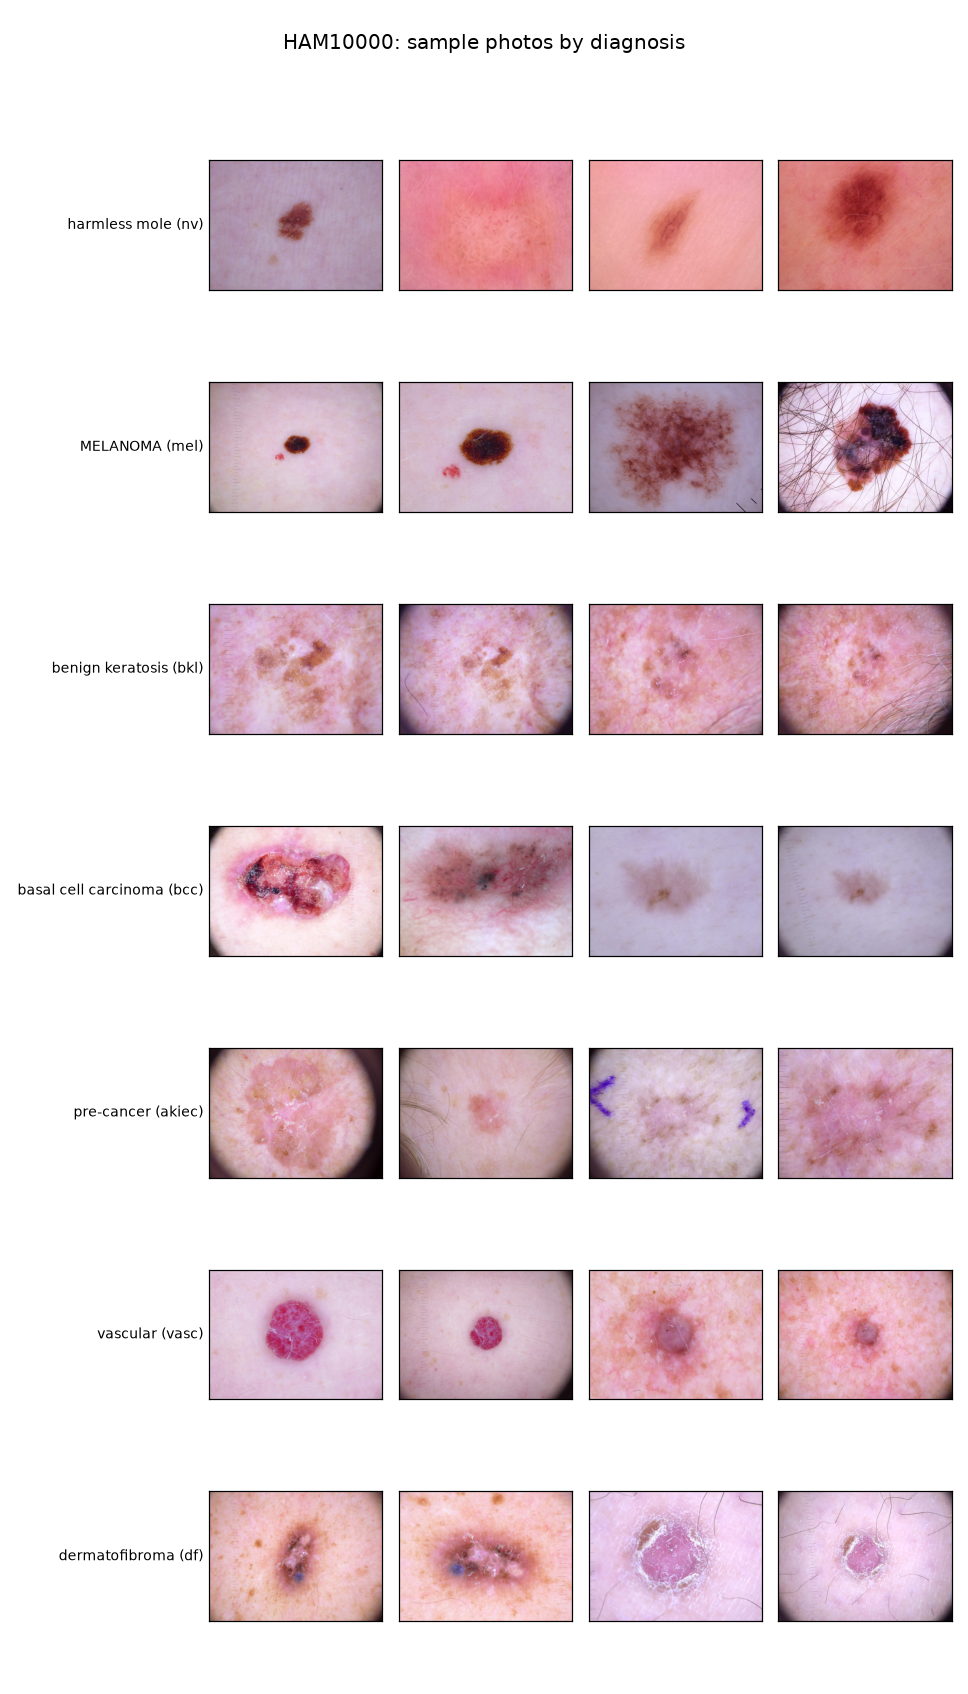
\includegraphics[width=0.85\linewidth]{figures/sample_photos.png}
\Description{Grid of example HAM10000 skin-lesion images, four per class.}
\caption{HAM10000 examples---clean, magnified, centred, the easy condition our
study degrades.}
\label{fig:samples}
\end{figure}

\section{Methodology}
Fig.~\ref{fig:pipeline} summarises both pipelines.

\begin{figure}[t]
\centering
\begin{tikzpicture}[font=\footnotesize,
  box/.style={draw, rounded corners, align=center, minimum height=6mm, inner sep=2pt},
  >={Stealth[length=1.6mm]}]
\node[box] (img) {Skin image\\(+ optional corruption)};
\node[box, above right=1mm and 7mm of img] (enet) {EfficientNet-B0\\(fine-tuned)};
\node[box, below right=1mm and 7mm of img] (dino) {DINOv2\\(frozen)};
\node[box, right=6mm of enet] (co) {label, softmax\\confidence};
\node[box, right=6mm of dino] (cr) {label, distance\\confidence};
\node[box, right=6mm of $(co)!0.5!(cr)$] (ev) {Evaluation};
\draw[->] (img) -- (enet); \draw[->] (img) -- (dino);
\draw[->] (enet) -- (co); \draw[->] (dino) -- (cr);
\draw[->] (co) -- (ev); \draw[->] (cr) -- (ev);
\end{tikzpicture}
\Description{Two pipelines: a classifier and a retrieval model sharing inputs and evaluation.}
\caption{The classifier (top) and retrieval (bottom) pipelines share the same
inputs and evaluation.}
\label{fig:pipeline}
\end{figure}

\subsection{Classifier}
An ImageNet-pretrained EfficientNet-B0~\citep{tan2019} with a fresh seven-way
head is fine-tuned with class-weighted cross-entropy:
\begin{equation}
\mathcal{L} = -\frac{1}{N}\sum_{i=1}^{N} w_{y_i}\log p_{i,y_i},
\qquad w_c=\frac{N}{C\,n_c},
\end{equation}
with $C{=}7$, $n_c$ the class count. Confidence is $\max_c p_{i,c}$.

\subsection{Retrieval}
Each training image is embedded by a frozen DINOv2 ViT-S/14
($\phi(\cdot)\in\mathbb{R}^{384}$)~\citep{oquab2024dinov2} and $L_2$-normalised.
For a query $q$, $s_j=\hat\phi_q^\top\hat\phi_j$, and over its $k$ nearest
neighbours $\mathcal{N}_k(q)$:
\begin{equation}
V_c(q)=\frac{1}{n_c}\!\!\sum_{j\in\mathcal{N}_k(q)}\!\! s_j\,\mathbb{1}[y_j=c],
\qquad \hat y=\arg\max_c V_c(q).
\end{equation}
Two confidence signals are compared: vote share
$V_{\hat y}/\sum_c V_c$, and a distance signal
$d(q)=\tfrac{1}{k}\sum_{j\in\mathcal{N}_k(q)} s_j$ mapped to a probability by an
isotonic regressor $g$~\citep{zadrozny2002} fit on a \emph{degraded} validation
set: $\mathrm{conf}(q)=g(d(q))$. Predictions are identical; only confidence
differs (Alg.~\ref{alg:ret}).

\begin{algorithm}[t]
\caption{Retrieval classification with distance confidence}
\label{alg:ret}
\begin{algorithmic}[1]
\Require query $q$; library $\{(\hat\phi_j,y_j)\}$; $k$; counts $n_c$; isotonic $g$
\State $\hat\phi_q \gets \phi(q)/\lVert\phi(q)\rVert$;\ \ $s_j \gets \hat\phi_q^\top\hat\phi_j$
\State $\mathcal{N}_k \gets$ top-$k$ by $s_j$
\State $V_c \gets \frac{1}{n_c}\sum_{j\in\mathcal{N}_k} s_j\,\mathbb{1}[y_j{=}c]$;\ \ $\hat y \gets \arg\max_c V_c$
\State $d \gets \frac{1}{k}\sum_{j\in\mathcal{N}_k} s_j$;\ \ $\mathrm{conf}\gets g(d)$
\State \Return $\hat y,\ \mathrm{conf}$
\end{algorithmic}
\end{algorithm}

\subsection{Corruptions and metrics}
Test images are degraded at three severities for five corruptions (blur, JPEG,
low light, noise, rotation), following~\citep{hendrycks2019}. We report balanced
accuracy, melanoma recall, ECE with reliability diagrams~\citep{guo2017}, and OOD
AUROC using maximum softmax probability~\citep{hendrycks2017} for the classifier
and mean neighbour similarity for retrieval, all with bootstrap 95\% CIs
(2{,}000 resamples).

\section{Experimental Setup}
Inputs are $224\times224$, ImageNet-normalised. The classifier trains 5 epochs
with AdamW (lr $10^{-4}$), batch 32, mixed precision, best epoch by validation
balanced accuracy. Retrieval uses $k{=}5$ (validation-selected) DINOv2 features,
no training. The isotonic calibrator is fit on a degraded 600-image validation
subset. All runs use one NVIDIA RTX 4050 GPU in PyTorch with fixed seed 42; code
and the exact split are released.

\section{Results}
\subsection{Clean images}
The classifier leads on clean data (Table~\ref{tab:clean}); a majority-class
baseline scores 0.668 accuracy but 0.143 balanced accuracy and zero melanoma
recall. The two models' clean melanoma-recall CIs overlap, so they are
\emph{not} significantly different on that class on clean images.

\begin{table}[t]
\caption{Clean HAM10000 test set (1{,}502 images), 95\% CIs.}
\label{tab:clean}
\centering
\begin{tabular}{lccc}
\toprule
Model & Accuracy & Balanced acc. & Melanoma recall\\
\midrule
Majority (nv) & 0.668 & 0.143 & 0.000\\
Retrieval     & 0.609 & 0.525\,{\footnotesize[.47,.58]} & 0.473\,{\footnotesize[.40,.55]}\\
Classifier    & \textbf{0.762} & \textbf{0.745}\,{\footnotesize[.70,.79]} & \textbf{0.557}\,{\footnotesize[.48,.63]}\\
\bottomrule
\end{tabular}
\end{table}

\subsection{Degradation hides a melanoma collapse}
Balanced accuracy is mixed (Fig.~\ref{fig:balacc}): the classifier leads under
blur and JPEG but nosedives under low light, noise, and rotation, where
retrieval overtakes. Melanoma recall (Fig.~\ref{fig:melrec},
Table~\ref{tab:melsevere}) is decisive: the classifier collapses to near zero
under every corruption while retrieval holds at 34--50\%. Even under blur and
JPEG the classifier misses 96--99\% of melanomas.

\begin{table}[t]
\caption{Melanoma recall at the most severe corruption.}
\label{tab:melsevere}
\centering
\begin{tabular}{lcc}
\toprule
Corruption (severe) & Classifier & Retrieval\\
\midrule
Low light & 0.00 & 0.50\\
Noise     & 0.00 & 0.49\\
Blur      & 0.04 & 0.40\\
JPEG      & 0.01 & 0.34\\
Rotation  & 0.08 & 0.50\\
\bottomrule
\end{tabular}
\end{table}

\begin{figure}[t]
\centering
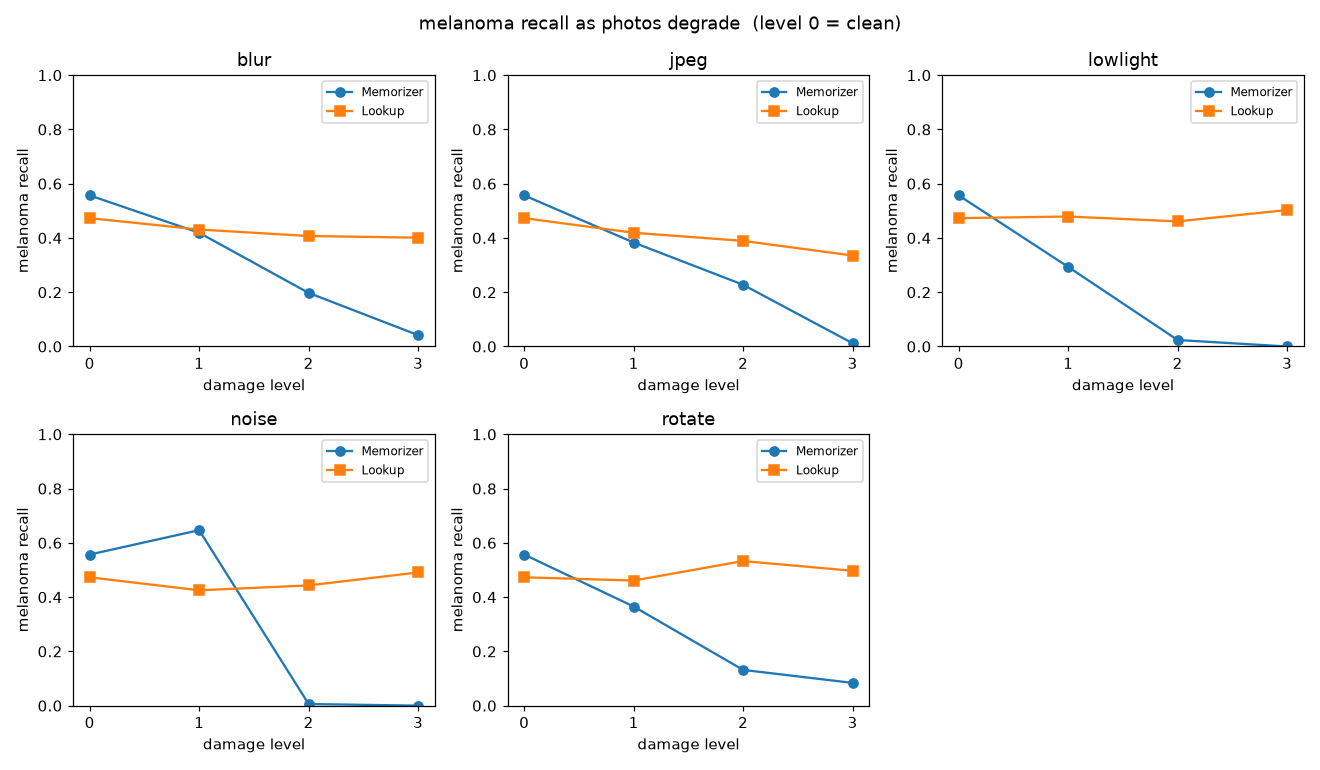
\includegraphics[width=\linewidth]{figures/degradation_melanoma_recall.png}
\Description{Melanoma recall versus corruption severity for both models.}
\caption{Melanoma recall as images degrade. The classifier (blue) collapses
toward zero; retrieval (orange) stays at 40--50\%.}
\label{fig:melrec}
\end{figure}

\begin{figure}[t]
\centering
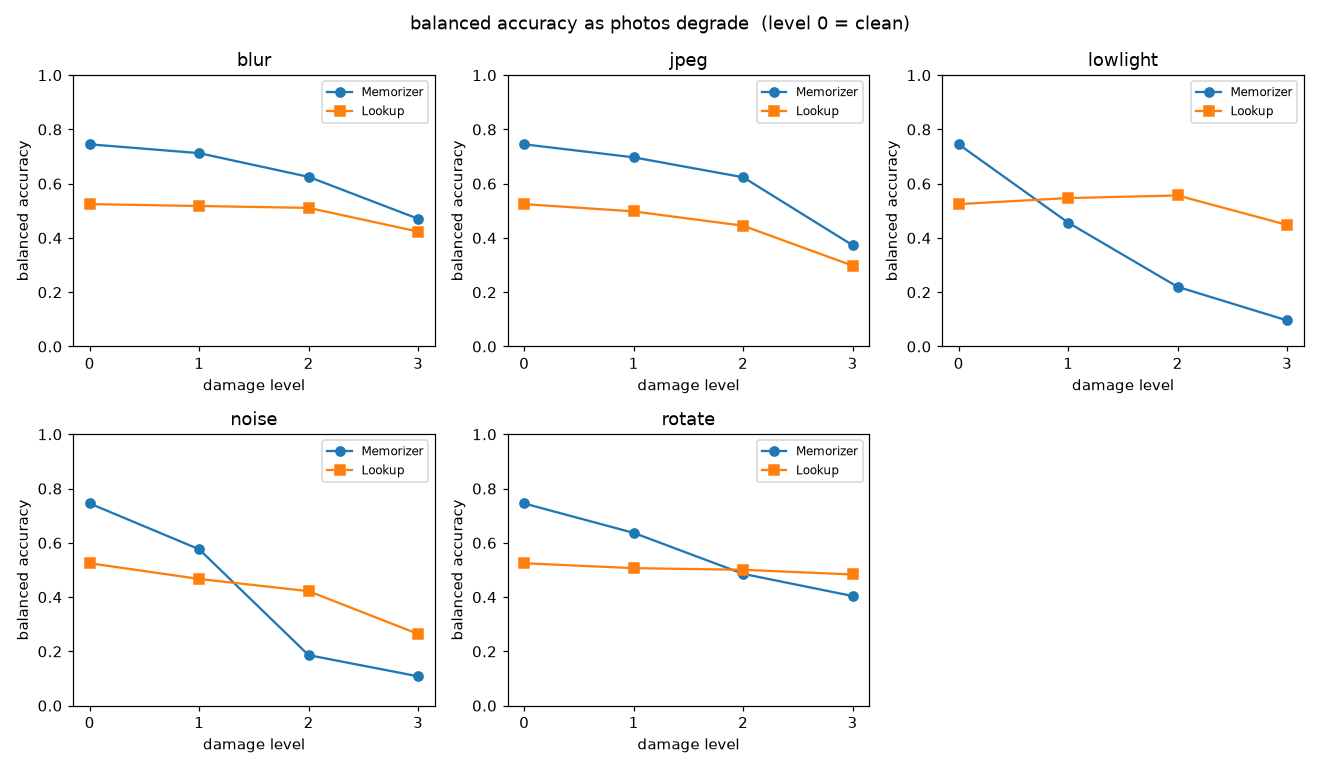
\includegraphics[width=\linewidth]{figures/degradation_balanced_accuracy.png}
\Description{Balanced accuracy versus corruption severity for both models.}
\caption{Balanced accuracy as images degrade---an honestly mixed aggregate
picture.}
\label{fig:balacc}
\end{figure}

\subsection{Calibration and confidence-signal ablation}
Table~\ref{tab:ece} ablates the confidence signal. Vote share is badly
overconfident and worsens under corruption; the distance signal is
best-calibrated and \emph{improves} under corruption
(Fig.~\ref{fig:reliab}). A neighbour-count ablation on validation balanced
accuracy gives 0.379, 0.513, 0.511, 0.511, 0.508 for $k{=}1,5,9,15,25$; we use
$k{=}5$.

\begin{table}[t]
\caption{Ablation: expected calibration error (lower = more honest).}
\label{tab:ece}
\centering
\begin{tabular}{lcc}
\toprule
Confidence signal & Clean & Heavily degraded\\
\midrule
Classifier softmax        & 0.08 & 0.14\\
Retrieval, vote share     & 0.23 & 0.31\\
Retrieval, distance (ours)& \textbf{0.05} & \textbf{0.03}\\
\bottomrule
\end{tabular}
\end{table}

\begin{figure}[t]
\centering
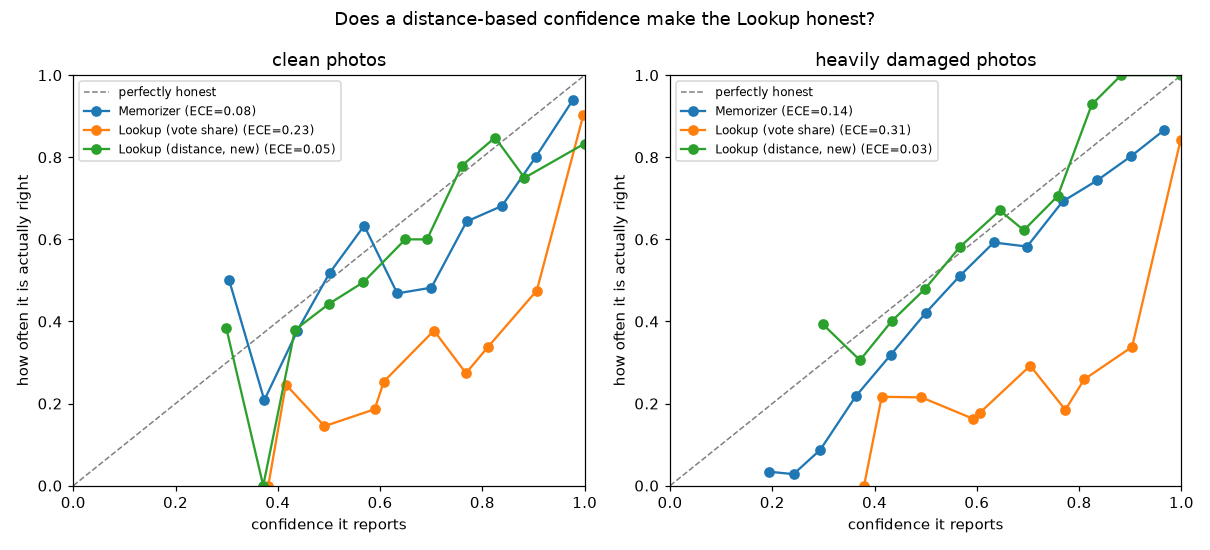
\includegraphics[width=\linewidth]{figures/calibration_lookup_reliability.png}
\Description{Reliability diagrams comparing confidence signals, clean and degraded.}
\caption{Reliability diagrams. The distance-based retrieval confidence (green)
hugs the diagonal; vote share (orange) sits far below it.}
\label{fig:reliab}
\end{figure}

\subsection{An honest negative: selective prediction}
Abstaining on the least-confident inputs raises overall accuracy on the retained
set, and the classifier's softmax triages overall accuracy \emph{better} than
retrieval's distance confidence. However, abstention does \emph{not} raise
melanoma recall for retrieval (near 0.45 on degraded images at all referral
rates): a well-calibrated score is not necessarily a good per-error ranking
signal.

\subsection{Real-world smartphone photos}
On PAD-UFES-20 (no retraining) both models lose accuracy
(Table~\ref{tab:pad})---expected for the modality shift. Yet retrieval catches
$3.5\times$ more melanomas (0.404 vs.\ 0.115, non-overlapping CIs), and its
similarity separates familiar HAM from unfamiliar PAD at AUROC 0.937 versus
0.720 for the classifier's softmax (Fig.~\ref{fig:ood}).

\begin{table}[t]
\caption{Real smartphone photos (PAD-UFES-20, 2{,}106 images), 95\% CIs.}
\label{tab:pad}
\centering
\begin{tabular}{lccc}
\toprule
Model & Accuracy & Melanoma recall & OOD AUROC\\
\midrule
Classifier & 0.290 & 0.115\,{\footnotesize[.04,.21]} & 0.720\,{\footnotesize[.70,.74]}\\
Retrieval  & 0.273 & \textbf{0.404}\,{\footnotesize[.27,.54]} & \textbf{0.937}\,{\footnotesize[.93,.95]}\\
\bottomrule
\end{tabular}
\end{table}

\begin{figure}[t]
\centering
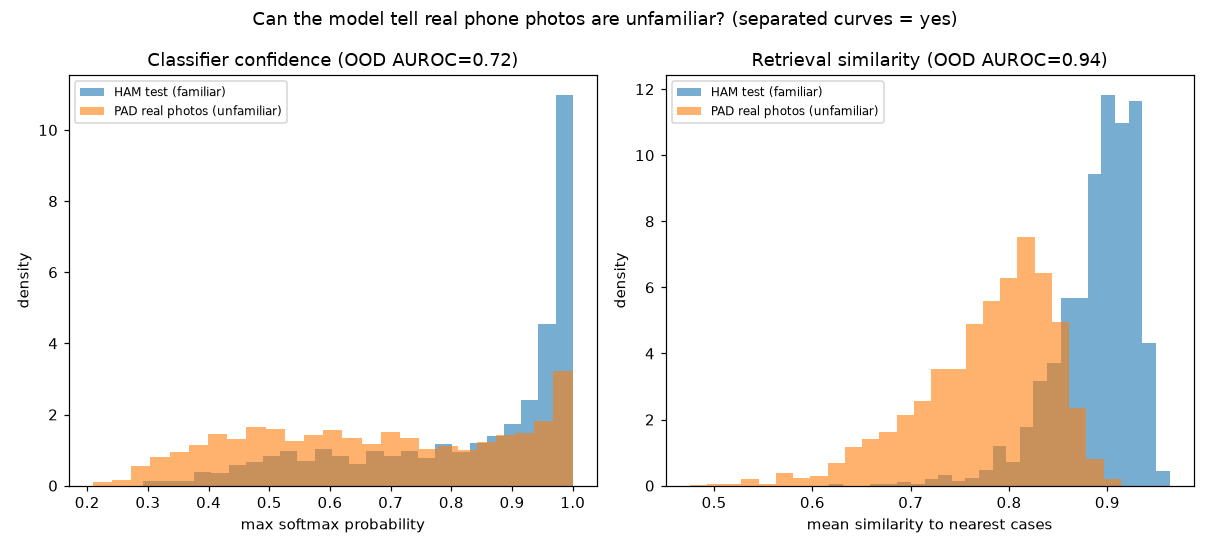
\includegraphics[width=\linewidth]{figures/pad_ood_detection.png}
\Description{Signal distributions for familiar HAM versus unfamiliar PAD images.}
\caption{Familiar (HAM) vs.\ unfamiliar (real PAD) signals. Classifier
confidence (left) overlaps; retrieval similarity (right) separates them.}
\label{fig:ood}
\end{figure}

\subsection{Error analysis}
Fig.~\ref{fig:neigh} shows, for melanoma queries, the nearest stored cases the
retrieval model consults. Correct cases sit beside melanomas; missed cases sit
beside benign look-alikes---transparency a classifier cannot offer.

\begin{figure}[t]
\centering
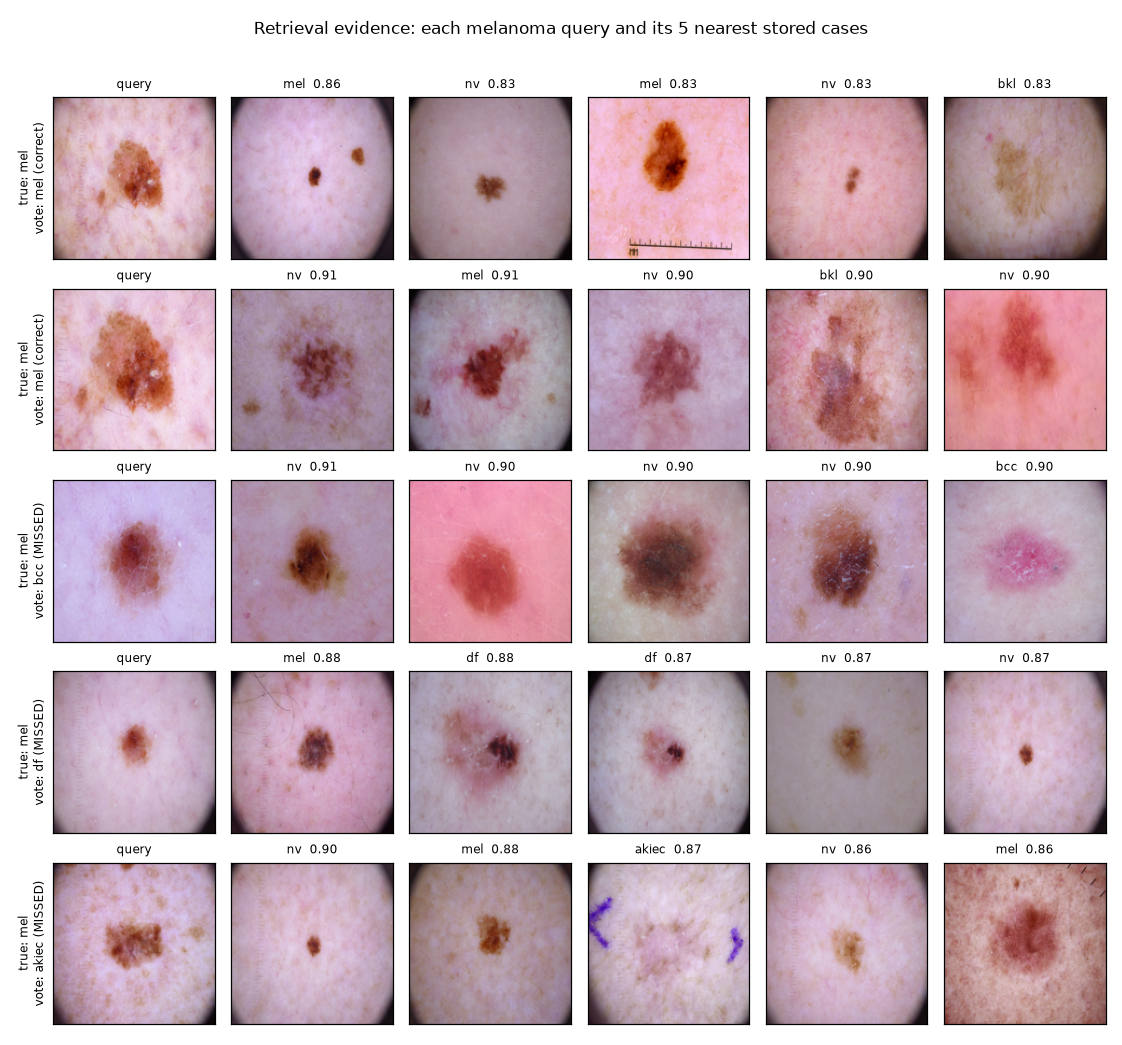
\includegraphics[width=\linewidth]{figures/retrieval_neighbours.png}
\Description{Melanoma queries with their five nearest retrieved cases and labels.}
\caption{Retrieval evidence: each melanoma query with its five nearest stored
cases. Rows 1--2 are voted correctly; rows 3--5 are missed.}
\label{fig:neigh}
\end{figure}

\section{Discussion}
Screening models should be judged by trust, not clean-set accuracy. A classifier
more accurate on curated data can fail silently on the malignant class under
degradation while staying confident. Retrieval trades clean-image accuracy for
graceful melanoma-recall degradation and, given a distance-based confidence,
honest uncertainty that survives shift and flags unfamiliar inputs. The
calibration finding is methodological: for retrieval the confidence definition
determines honesty under shift. The selective-prediction negative shows
calibration improves a score's \emph{value} without necessarily improving its
\emph{ranking} of errors.

\section{Limitations}
Controlled corruptions are simulated, though we add a real smartphone dataset.
Training uses a single source; the modality shift is large, so PAD accuracy is
low for both models and neither is deployable. The retrieval fingerprint is a
general (not skin-specific) embedding, and the study was single-GPU and short.

\section{Conclusion and Future Work}
A retrieval model with a distance-based, shift-calibrated confidence is
simultaneously more robust on melanoma and more honest about its uncertainty
than a strong classifier, whereas aggregate accuracy hides the classifier's
silent failures. Future work: skin-specific embeddings (e.g.,
PanDerm~\citep{yan2025panderm}, BiomedCLIP~\citep{zhang2025biomedclip}); fairness
across skin tones (PAD-UFES-20 has Fitzpatrick labels); error-aware referral;
and more real-world datasets. Code and the exact split are available at
\url{https://github.com/nishankhareln/skin_research}.

\bibliographystyle{ACM-Reference-Format}
\begin{thebibliography}{99}
\bibitem[Esteva et al.(2017)]{esteva2017} A. Esteva et al. 2017. Dermatologist-level classification of skin cancer with deep neural networks. \textit{Nature} 542, 115--118.
\bibitem[Tschandl et al.(2018)]{tschandl2018} P. Tschandl, C. Rosendahl, and H. Kittler. 2018. The HAM10000 dataset. \textit{Scientific Data} 5, 180161.
\bibitem[Pacheco et al.(2020)]{pacheco2020} A. G. C. Pacheco et al. 2020. PAD-UFES-20: A skin lesion dataset from smartphones. \textit{Data in Brief} 32, 106221.
\bibitem[Codella et al.(2018)]{codella2018} N. C. F. Codella et al. 2018. Skin lesion analysis toward melanoma detection: A challenge at ISIC. In \textit{IEEE ISBI}.
\bibitem[Tan and Le(2019)]{tan2019} M. Tan and Q. Le. 2019. EfficientNet: Rethinking model scaling for CNNs. In \textit{ICML}.
\bibitem[Oquab et al.(2024)]{oquab2024dinov2} M. Oquab et al. 2024. DINOv2: Learning robust visual features without supervision. \textit{TMLR}.
\bibitem[Zhang et al.(2025)]{zhang2025biomedclip} S. Zhang et al. 2025. BiomedCLIP: A multimodal biomedical foundation model. \textit{NEJM AI} 2, 1.
\bibitem[Yan et al.(2025)]{yan2025panderm} S. Yan et al. 2025. A multimodal vision foundation model for clinical dermatology. \textit{Nature Medicine} 31, 8, 2691--2702.
\bibitem[Hendrycks and Dietterich(2019)]{hendrycks2019} D. Hendrycks and T. Dietterich. 2019. Benchmarking neural network robustness to common corruptions. In \textit{ICLR}.
\bibitem[Maron et al.(2021)]{maron2021} R. C. Maron et al. 2021. A benchmark for neural network robustness in skin cancer classification. \textit{European Journal of Cancer} 155, 191--199.
\bibitem[Hu et al.(2024)]{hu2024diffusion} M. Hu et al. 2024. Diffusion model driven test-time image adaptation for robust skin lesion classification. arXiv:2405.11289.
\bibitem[Bissoto et al.(2022)]{bissoto2022artifact} A. Bissoto, C. Barata, E. Valle, and S. Avila. 2022. Artifact-based domain generalization of skin lesion models. In \textit{ECCV Workshops (ISIC)}.
\bibitem[Di Salvo et al.(2024)]{disalvo2024medmnistc} F. Di Salvo, S. Doerrich, and C. Ledig. 2024. MedMNIST-C: Benchmark and improved robustness via realistic corruptions. In \textit{MICCAI Workshop (ADSMI)}.
\bibitem[Guo et al.(2017)]{guo2017} C. Guo, G. Pleiss, Y. Sun, and K. Q. Weinberger. 2017. On calibration of modern neural networks. In \textit{ICML}.
\bibitem[Naeini et al.(2015)]{naeini2015} M. P. Naeini, G. Cooper, and M. Hauskrecht. 2015. Obtaining well calibrated probabilities using Bayesian binning. In \textit{AAAI}.
\bibitem[Zadrozny and Elkan(2002)]{zadrozny2002} B. Zadrozny and C. Elkan. 2002. Transforming classifier scores into accurate multiclass probability estimates. In \textit{ACM KDD}.
\bibitem[Fayyad et al.(2024)]{fayyad2024conformal} J. Fayyad, S. Alijani, and H. Najjaran. 2024. Empirical validation of conformal prediction for trustworthy skin lesions classification. \textit{Computer Methods and Programs in Biomedicine} 253, 108231.
\bibitem[Penso et al.(2024)]{penso2024calibration} C. Penso, L. Frenkel, and J. Goldberger. 2024. Confidence calibration of a medical imaging classification system robust to label noise. \textit{IEEE TMI} 43, 6, 2050--2060.
\bibitem[Sambyal et al.(2023)]{sambyal2023understanding} A. S. Sambyal, U. Niyaz, N. C. Krishnan, and D. R. Bathula. 2023. Understanding calibration of deep neural networks for medical image classification. \textit{Computer Methods and Programs in Biomedicine} 242, 107816.
\bibitem[Gassner et al.(2023)]{gassner2023secbir} M. Gassner et al. 2023. Saliency-enhanced content-based image retrieval for diagnosis support in dermatology: Reader study. \textit{JMIR Dermatology} 6, e42129.
\bibitem[Gupta et al.(2023)]{gupta2023mednn} D. Gupta, R. Loane, S. Gayen, and D. Demner-Fushman. 2023. Medical image retrieval via nearest neighbor search on pre-trained image features. \textit{Knowledge-Based Systems} 278, 110907.
\bibitem[He et al.(2022)]{he2022demal} X. He, Y. Wang, S. Zhao, and X. Chen. 2022. Deep metric attention learning for skin lesion classification in dermoscopy images. \textit{Complex \& Intelligent Systems} 8, 2, 1487--1504.
\bibitem[Hendrycks and Gimpel(2017)]{hendrycks2017} D. Hendrycks and K. Gimpel. 2017. A baseline for detecting misclassified and out-of-distribution examples. In \textit{ICLR}.
\bibitem[Zimmerer et al.(2022)]{zimmerer2022mood} D. Zimmerer et al. 2022. MOOD 2020: A public benchmark for OOD detection on medical images. \textit{IEEE TMI} 41, 10.
\bibitem[Gutbrod et al.(2025)]{gutbrod2025openmibood} M. Gutbrod, D. Rauber, D. W. Nunes, and C. Palm. 2025. OpenMIBOOD: Open medical imaging benchmarks for OOD detection. In \textit{IEEE/CVF CVPR}.
\bibitem[Huang et al.(2022)]{huang2022multiscale} Z. Huang, T. Wang, Y. Cai, and L. Liang. 2022. A multi-scale framework for OOD detection in dermoscopic images. In \textit{ML4CS}.
\bibitem[Abhishek et al.(2025)]{abhishek2025dermamnist} K. Abhishek, A. Jain, and G. Hamarneh. 2025. Investigating the quality of DermaMNIST and Fitzpatrick17k datasets. \textit{Scientific Data} 12, 1, 196.
\bibitem[Geifman and El-Yaniv(2017)]{geifman2017} Y. Geifman and R. El-Yaniv. 2017. Selective classification for deep neural networks. In \textit{NeurIPS}.
\bibitem[Liu et al.(2022)]{liu2022ldu} J. Liu, B. Gallego, and S. Barbieri. 2022. Incorporating uncertainty in learning to defer for safe computer-aided diagnosis. \textit{Scientific Reports} 12, 1762.
\bibitem[Verma et al.(2023)]{verma2023multiexpert} R. Verma, D. Barrejon, and E. Nalisnick. 2023. Learning to defer to multiple experts. In \textit{AISTATS}.
\bibitem[Dvijotham et al.(2023)]{dvijotham2023codoc} K. Dvijotham et al. 2023. Enhancing reliability and accuracy of AI-enabled diagnosis via complementarity-driven deferral to clinicians. \textit{Nature Medicine} 29, 7.
\end{thebibliography}

\end{document}
